\subsubsection{ClientModel}

\textbf{GoIntentService}

\paragraph{Database}

\textbf{DBHelper}

Die vier nachfolgenden DBHelper erben ihren Konstruktor und ihre Methoden von SQLiteOpenHelper. Der Konstruktor definiert dabei den Namen und die Versionsnummer der Datenbank.
Mit der onCreate() Methode wird die SQLiteDatenbank mit den in FeedReaderContract definierten Spalten aufgebaut, wenn sie das erste Mal aufgerufen wird.
Mit onUpgrade() kann die Datenbank verändert und auf eine neue Versionsnummer hochgesetzt werden. Beispielsweise, wenn man nachträglich noch eine weitere Spalte hinzufügen oder ähnliche Veränderungen vornehmen möchte.
\begin{enumerate}
	\item
	\item
\end{enumerate}

\begin{figure}[H]
	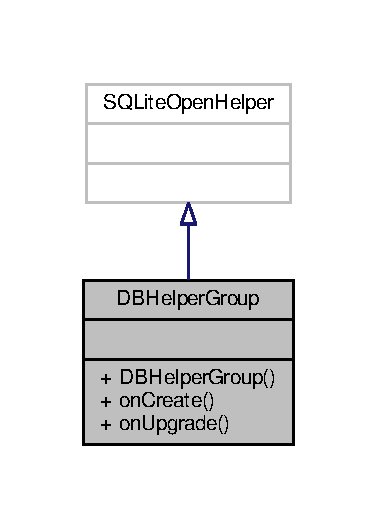
\includegraphics[scale = 1]{res/umlClasses/d_b_helper_group__coll__graph.pdf}
	\centering	
\end{figure}

\begin{figure}[H]
	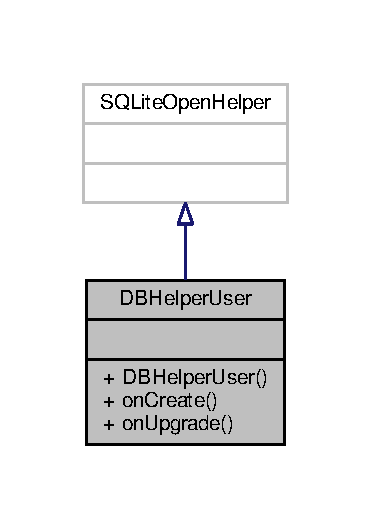
\includegraphics[scale = 1]{res/umlClasses/d_b_helper_user__coll__graph.pdf}
	\centering
\end{figure}

\begin{figure}[H]
	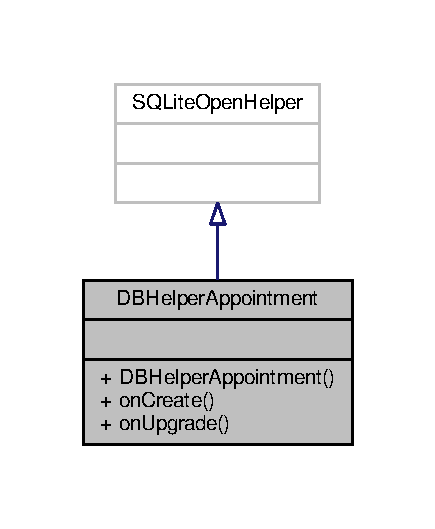
\includegraphics[scale = 1]{res/umlClasses/d_b_helper_appointment__coll__graph.pdf}
	\centering
\end{figure}

\begin{figure}[H]
	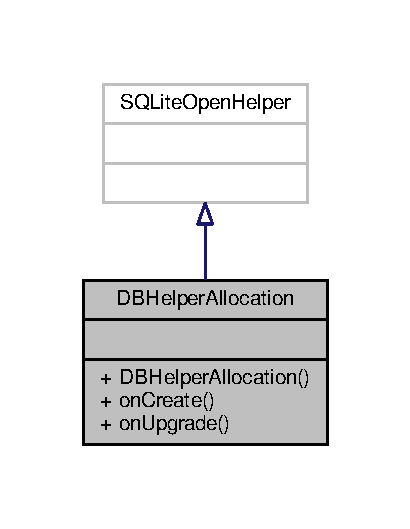
\includegraphics[scale = 1]{res/umlClasses/d_b_helper_allocation__coll__graph.pdf}
	\centering
\end{figure}



\textbf{FeedReaderContract}
\begin{figure}[H]
	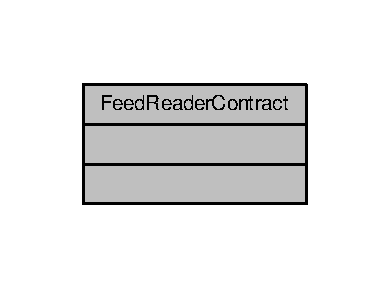
\includegraphics[scale = 1]{res/umlClasses/feed_reader_contract__coll__graph.pdf}
	\centering
\end{figure}
Die FeedReaderContract Klasse definiert in statischen Innenklassen wie die Tabellen der Datenbank aufgebaut sind. Jede der nachfolgenden FeedEntry Klassen implementiert dabei das interface BaseColumns.
CREATE ENTRIES definiert wie aus den zuvor definierten Namen der Spalten die Tabelle in genau dieser Reihenfolge aufgebaut wird.
DELETE ENTRIES löscht die definierten Einträge wieder.

\textbf{FeedEntyGroup}
\begin{figure}[H]
	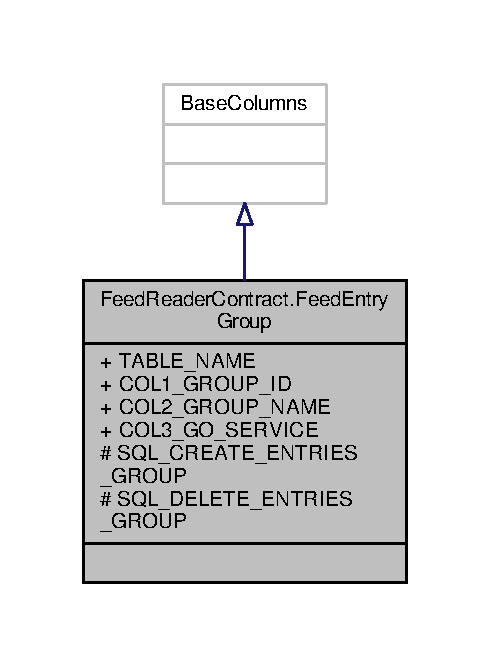
\includegraphics[scale = 1]{res/umlClasses/feed_reader_contract_group.pdf}
	\centering
\end{figure}
Die Innenklasse FeedEntryGroup definiert den Namen und die Spalten der Tabelle, welche die Gruppen auf dem Client speichert. 
Dabei steht in der ersten Spalte die eindeutige Gruppen ID (welche die Zeilen eindeutig unterscheidbar macht), in der zweiten Spalte der eindeutige Gruppenname und in der dritten Spalte, ob der GoService des aktuellen Benutzers für diese Gruppe aktiviert oder deaktiviert ist.
Wenn eine Gruppe gelöscht wird, dann wird auch ihr Eintrag in der Datenbank gelöscht.

\textbf{FeedEntyUser}
\begin{figure}[H]
	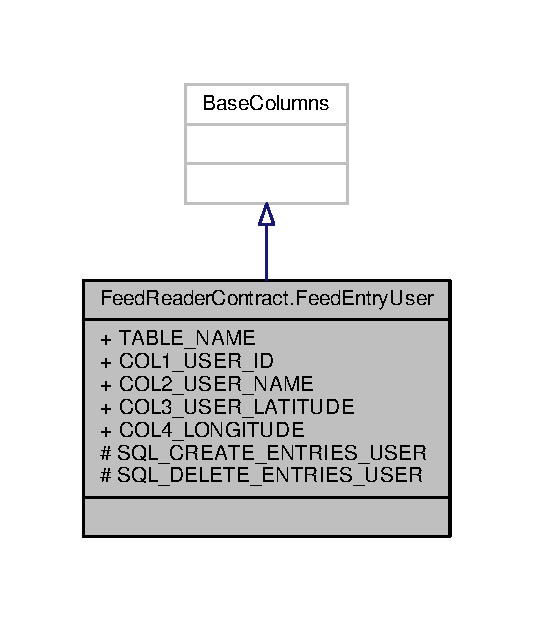
\includegraphics[scale = 1]{res/umlClasses/feed_reader_contract_user.pdf}
	\centering
\end{figure}
Die Innenklasse FeedEntryUser definiert den Namen und die Spalten der Tabelle, welche die Benutzer auf dem Client speichert. 
Dabei steht in der ersten Spalte die eindeutige Benutzer ID (welche die Zeilen eindeutig unterscheidbar macht), in der zweiten Spalte der Benutzername und in der dritten und vierten Spalte steht je ein Wert der zuletzt bekannten Gps Daten des jeweiligen Nutzers. 
Es werden nur Benutzer gespeichert mit denen der aktuelle Benutzer in mindestens einer gemeinsamen Gruppe ist.
\begin{enumerate}
	\item
	\item
\end{enumerate}


\textbf{FeedEntyAppointment}
\begin{figure}[H]
	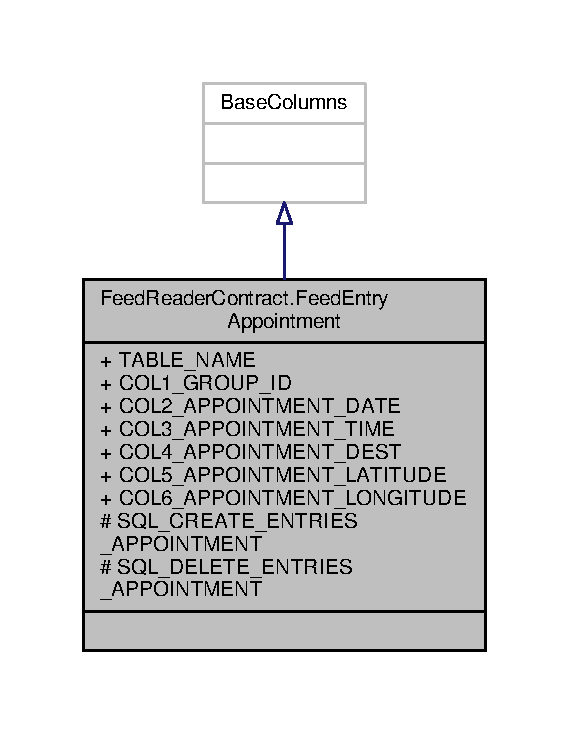
\includegraphics[scale = 1]{res/umlClasses/feed_reader_contract_appointment.pdf}
	\centering
\end{figure}
Die Innenklasse FeedEntryAppointment definiert den Namen und die Spalten der Tabelle, welche die Treffpunkte zu jeder Gruppe speichert. Jede Gruppe hat dabei nur eine Zeile, welche den Treffpunkt definiert. 
Dabei steht in der ersten Spalte die Gruppen id (welche die Zeilen eindeutig unterscheidbar macht), in der zweiten Spalte steht das Datum und in der dritten die Uhrzeit des Treffpunktes. In der vierten Spalte steht der Name des Zielortes und in der fünften und sechsten steht jeweils ein Wert der Gps Daten des Zielortes. 
Wenn sich der Treffpunkt der Gruppe ändert, dann werden die Werte des alten Treffpunktes überschrieben.
Sollte die die Gruppe des dazugehörigen Treffpunktes gelöscht werden, dann wird auch der Eintrag in dieser Tabelle gelöscht.
\begin{enumerate}
	\item
	\item
\end{enumerate}


\textbf{FeedEntyAllocation}
\begin{figure}[H]
	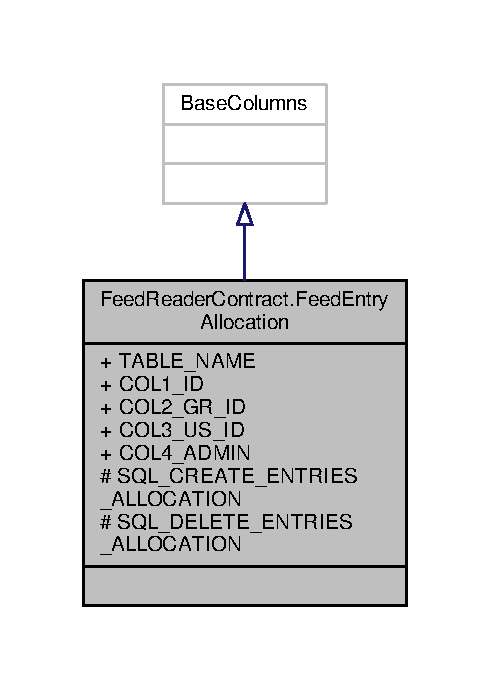
\includegraphics[scale = 1]{res/umlClasses/feed_reader_contract_allocation.pdf}
	\centering
\end{figure}
Die Innenklasse FeedEntryAllocation definiert den Namen und die Spalten der Tabelle, welche die jeweiligen Mitglieder jeder Gruppe speichert, in der der aktuelle Benutzer Mitglied ist. Zu jedem Mitglied wird vermerkt, ob dieses Administratorrechte hat.
Dabei steht in der ersten Spalte die Allocation id (welche die Zeilen eindeutig unterscheidbar macht und automatisch hochgezählt), in der zweiten Spalte steht die Gruppen id, in der dritten Spalte die Benutzer id und in der vierten Spalte, ob dieser Benutzer Gruppenadministrator ist oder nicht. 
Gruppen id wird für jedes Gruppenmitglied vermerkt, also kommt mehrmals vor, sobald mehr als ein Benutzer Mitglied dieser Gruppe ist. 
\begin{enumerate}
	\item
	\item
\end{enumerate}


\paragraph{ObjectStructure}

\textbf{GroupClient}
Die Klasse GroupClient definiert wie eine Gruppe auf dem Client aufgebaut ist und welche Funktionalität ihr zur Verfügung steht.
Beim Erstellen einer neuen Gruppe muss der Benutzer einen eindeutigen Namen wählen, wird dann Gruppenadministrator und kann neue Mitglieder einladen indem er mit createInviteLink() einen Link zu dieser Gruppe erstellt. Führt das Mitglied den Link aus, dann wird es entweder direkt über die Go-App zur Gruppe geleitet und hinzugefügt oder aufgefordert die Go-App zu installieren.
Der Gruppenadministrator kann andere Gruppenmitglieder auch zu Gruppenadministratoren machen.
Mit getAllGroupMemberNames() können die Namen aller Gruppenmitglieder in der Gruppe angezeigt werden.
Mit deleteGroupMember() kann der Administrator ein Gruppenmitglied entfernen und mit leaveGroup() kann ein Gruppenmitglied selbst die Gruppe verlassen.
Mit activateGoService() bzw. deaktivateGoService() kann der aktuelle Benutzer angeben, ob er in dieser Gruppe seine Position den anderen Mitgliedern mitteilen möchte. Ist der goService() aktiviert aber GPS Verfolgung am Mobiltelefon ausgeschaltet, dann wird die letzte bekannte Position angezeigt, zu welcher goService und GPS aktiviert waren.
Mit changeGroupName() kann der Administrator den Gruppennamen nachträglich verändern aber auch der neue Gruppenname muss eindeutig sein.
Mit den restlichen gettern können die Informationen zur Gruppe abgerufen werden. Mit getMember() wird unterschieden, welche App Ansicht der aktuellen Benutzer für die jeweilige Gruppe hat. Ist er Administrator, dann werden ihm die Funktionalitäten angezeigt, die nur ein Administrator hat. Wenn nicht, dann stehen Funktionen wie Mitglieder hinzufügen/ entfernen oder Treffpunkt festlegen gar nicht erst zur Verfügung.
\begin{enumerate}
	\item
	\item
\end{enumerate}


\textbf{UserComponent}
Dieses Interface ist die erste Komponente des Decorator pattern und definiert drei grundlegende Funktionen des Benutzers die jederzeit aufgerufen werden können. 
Mit getUserName() kann der Benutzername des aktuellen Nutzers visualisiert werden.
Mit getUserId() kann der Benutzer von anderen Gruppenmitgliedern unterschieden werden, da der Benutzername nicht eindeutig sein muss, die Id aber schon.
Mit getUserDeviceId() kann der Benutzer auf dem Server angelegt werden. Jede Gerätenummer kann nur einmal auf dem Server vorkommen, um Missbrauch der GoApp vorzubeugen.
\begin{enumerate}
	\item
	\item
\end{enumerate}


\textbf{SimpleUser}
Die SimpleUser Klasse implementiert das UserComponent Interface und besitzt eine zusätzliche changeUserName() Methode um den Benutzernamen nachträglich zu ändern. Der Benutzer ist ein SimpleUser Objekt, wenn er nicht in der Gruppenansicht ist und so weder einem Gruppenadministrator noch einem Gruppenmitglied
\begin{enumerate}
	\item
	\item
\end{enumerate}
 entspricht.

\textbf{UserDecorator}
Die UserDecorator Klasse ist eine abstrakte Klasse, die wie SimpleUser das UserComponent Interface implementiert. 
Mit getView() kann die Gruppenansicht bestimmt werden indem überprüft wird, ob der Benutzer in der aufgerufenen Gruppe nur Gruppenmitglied oder Administrator ist. Als Administrator stehen dem Benutzer zusätzliche Funktionen zur Verfügung, die dann in der Gruppenansicht angezeigt werden.
Mit getGpsObject() wird die aktuelle Position des Benutzers angefragt, sobald er seinen Go Button aktiviert hat.
\begin{enumerate}
	\item
	\item
\end{enumerate}


\textbf{GroupAdmin}
\begin{enumerate}
	\item
	\item
\end{enumerate}

\textbf{GroupMember}


\textbf{GoStatus}

\textbf{Link}

\textbf{GpsObject}


\textbf{Appointment}

\textbf{AppointmentDate}

\textbf{AppointmentDestination}








